\subsection{Giao diện xem trước bảng khảo sát}

\begin{figure}[H]
    \centering
    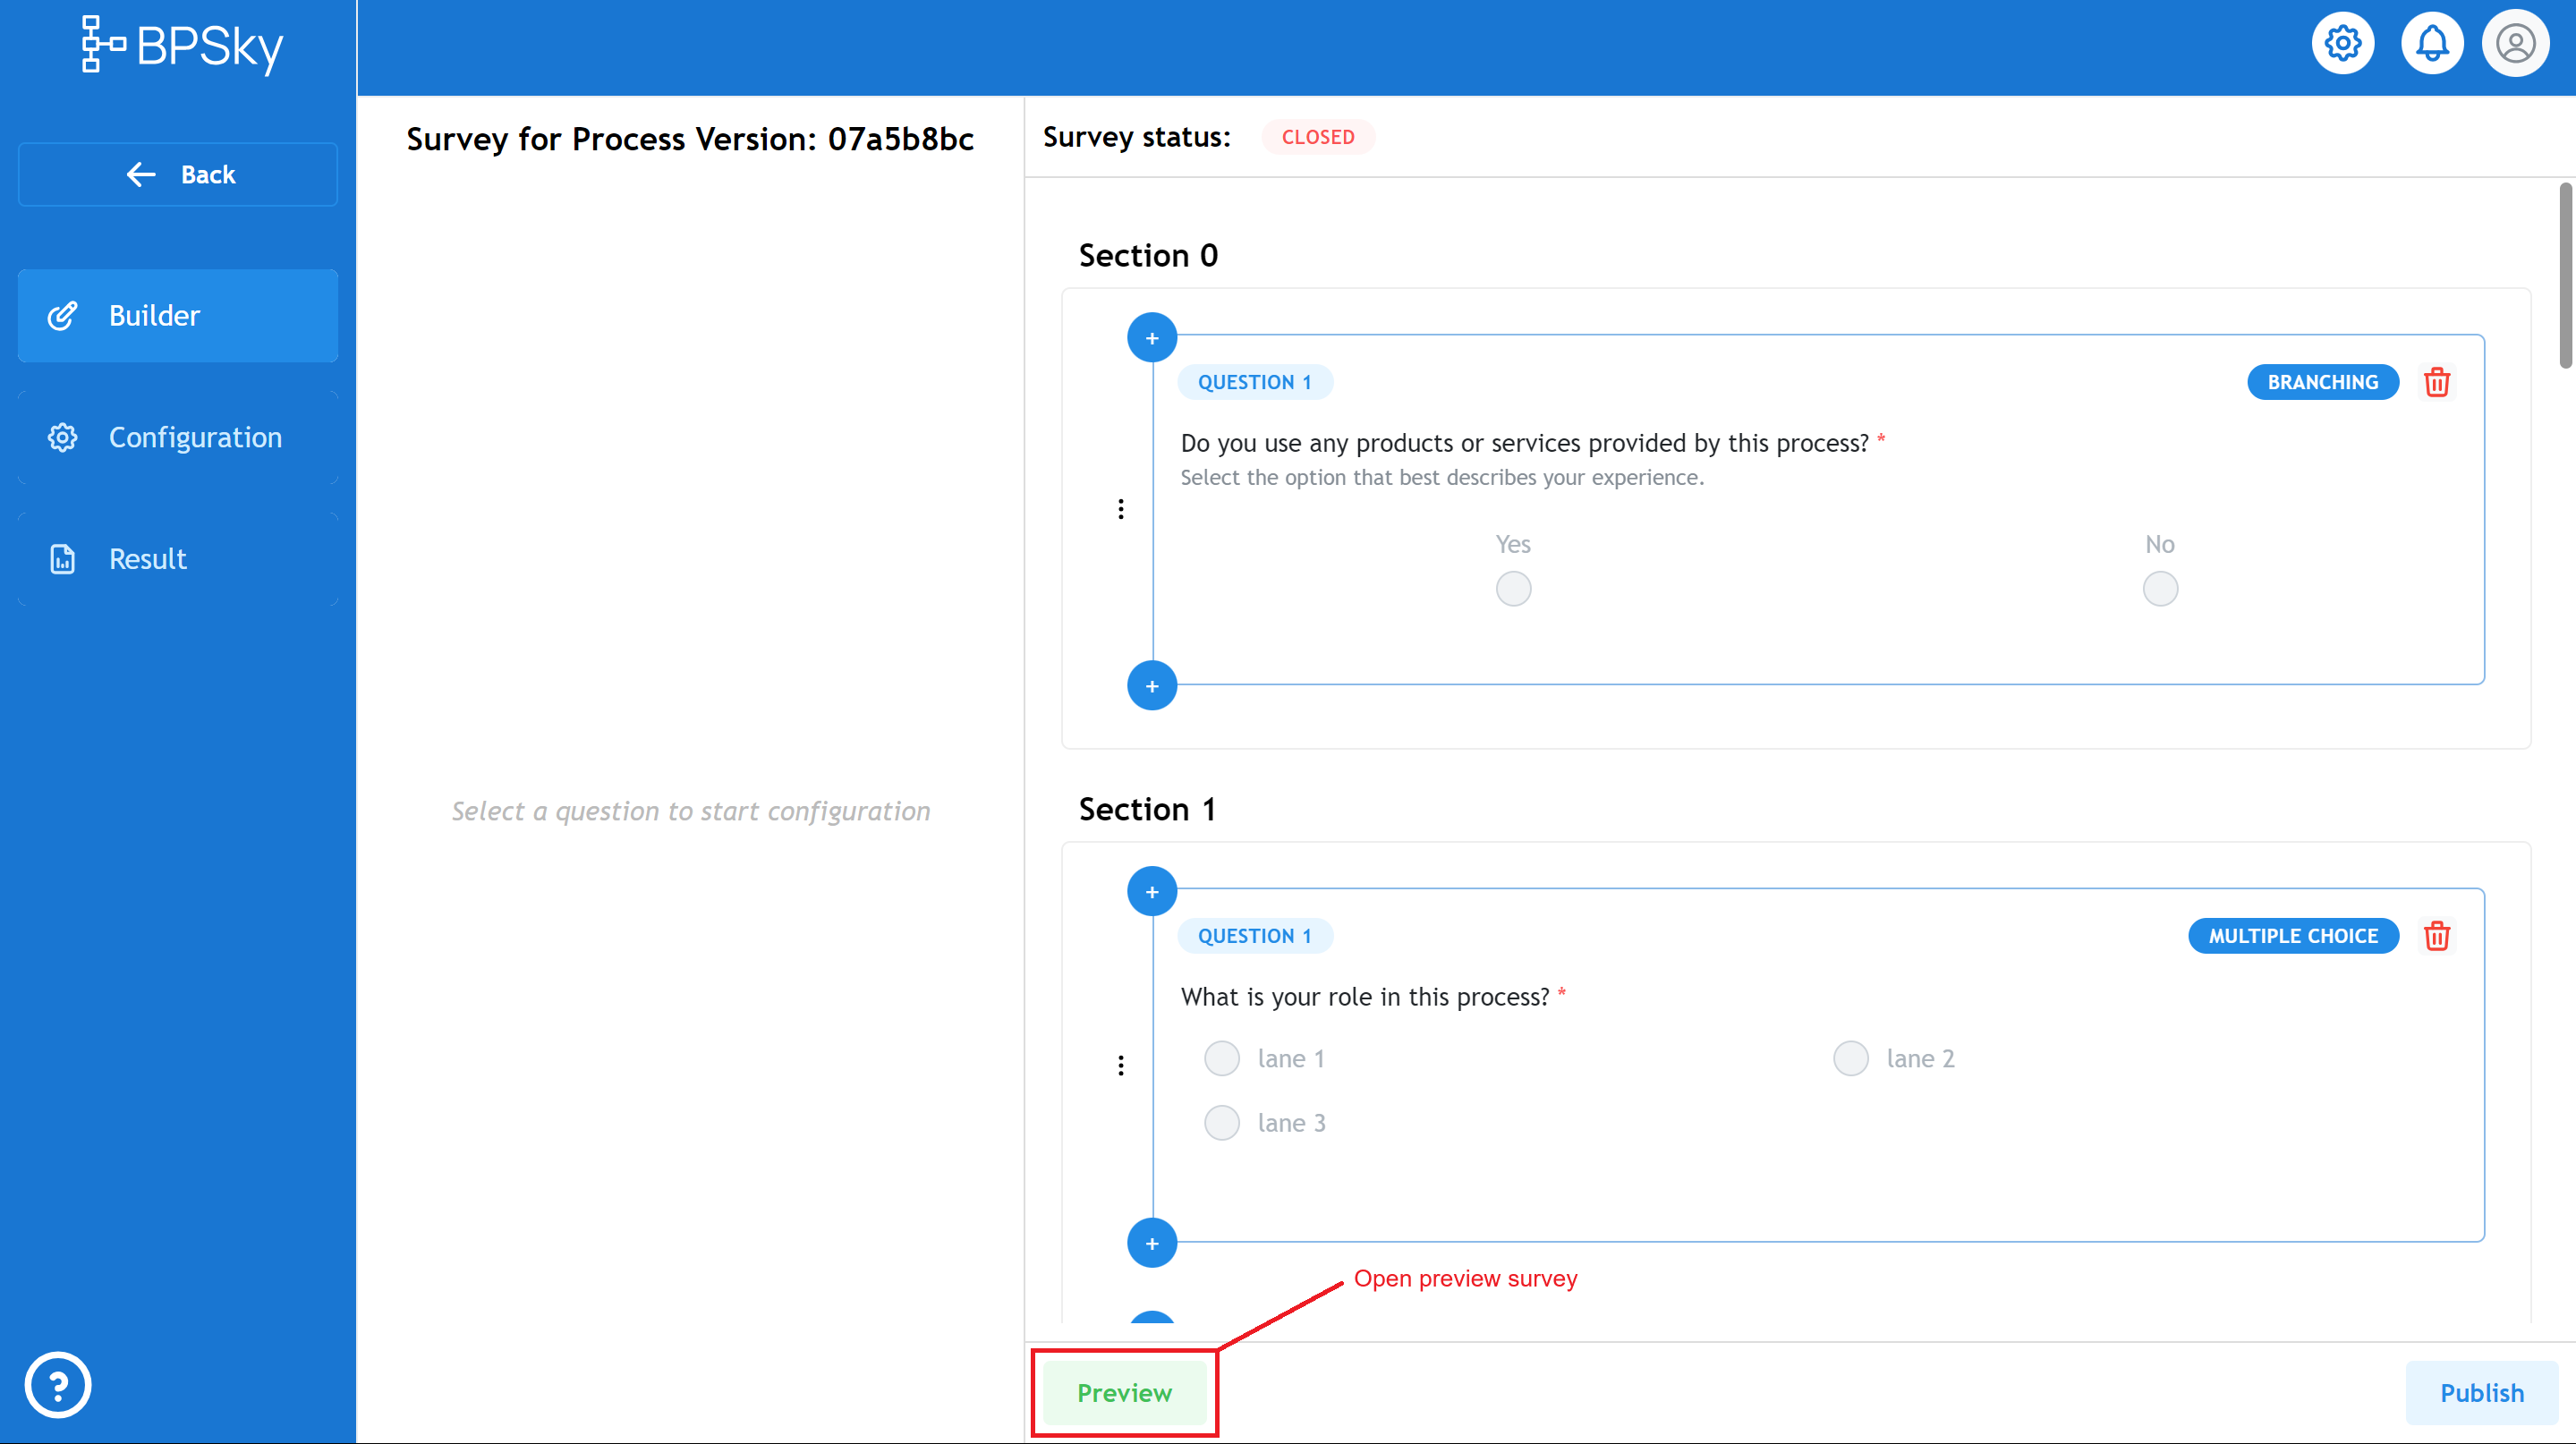
\includegraphics[ width = \linewidth]{Content/Hiện thực hệ thống/documents/Hiện thực giao diện người dùng/images/SurveyPreview.png}
    \vspace{0.5cm}
    \caption{Giao diện xem trước bảng khảo sát}
    \label{fig: Giao diện xem trước bảng khảo sát}
\end{figure}

Người dùng có thể chọn nút Preview để mở phiên bản preview của bảng khảo sát.

\begin{figure}[H]
    \centering
    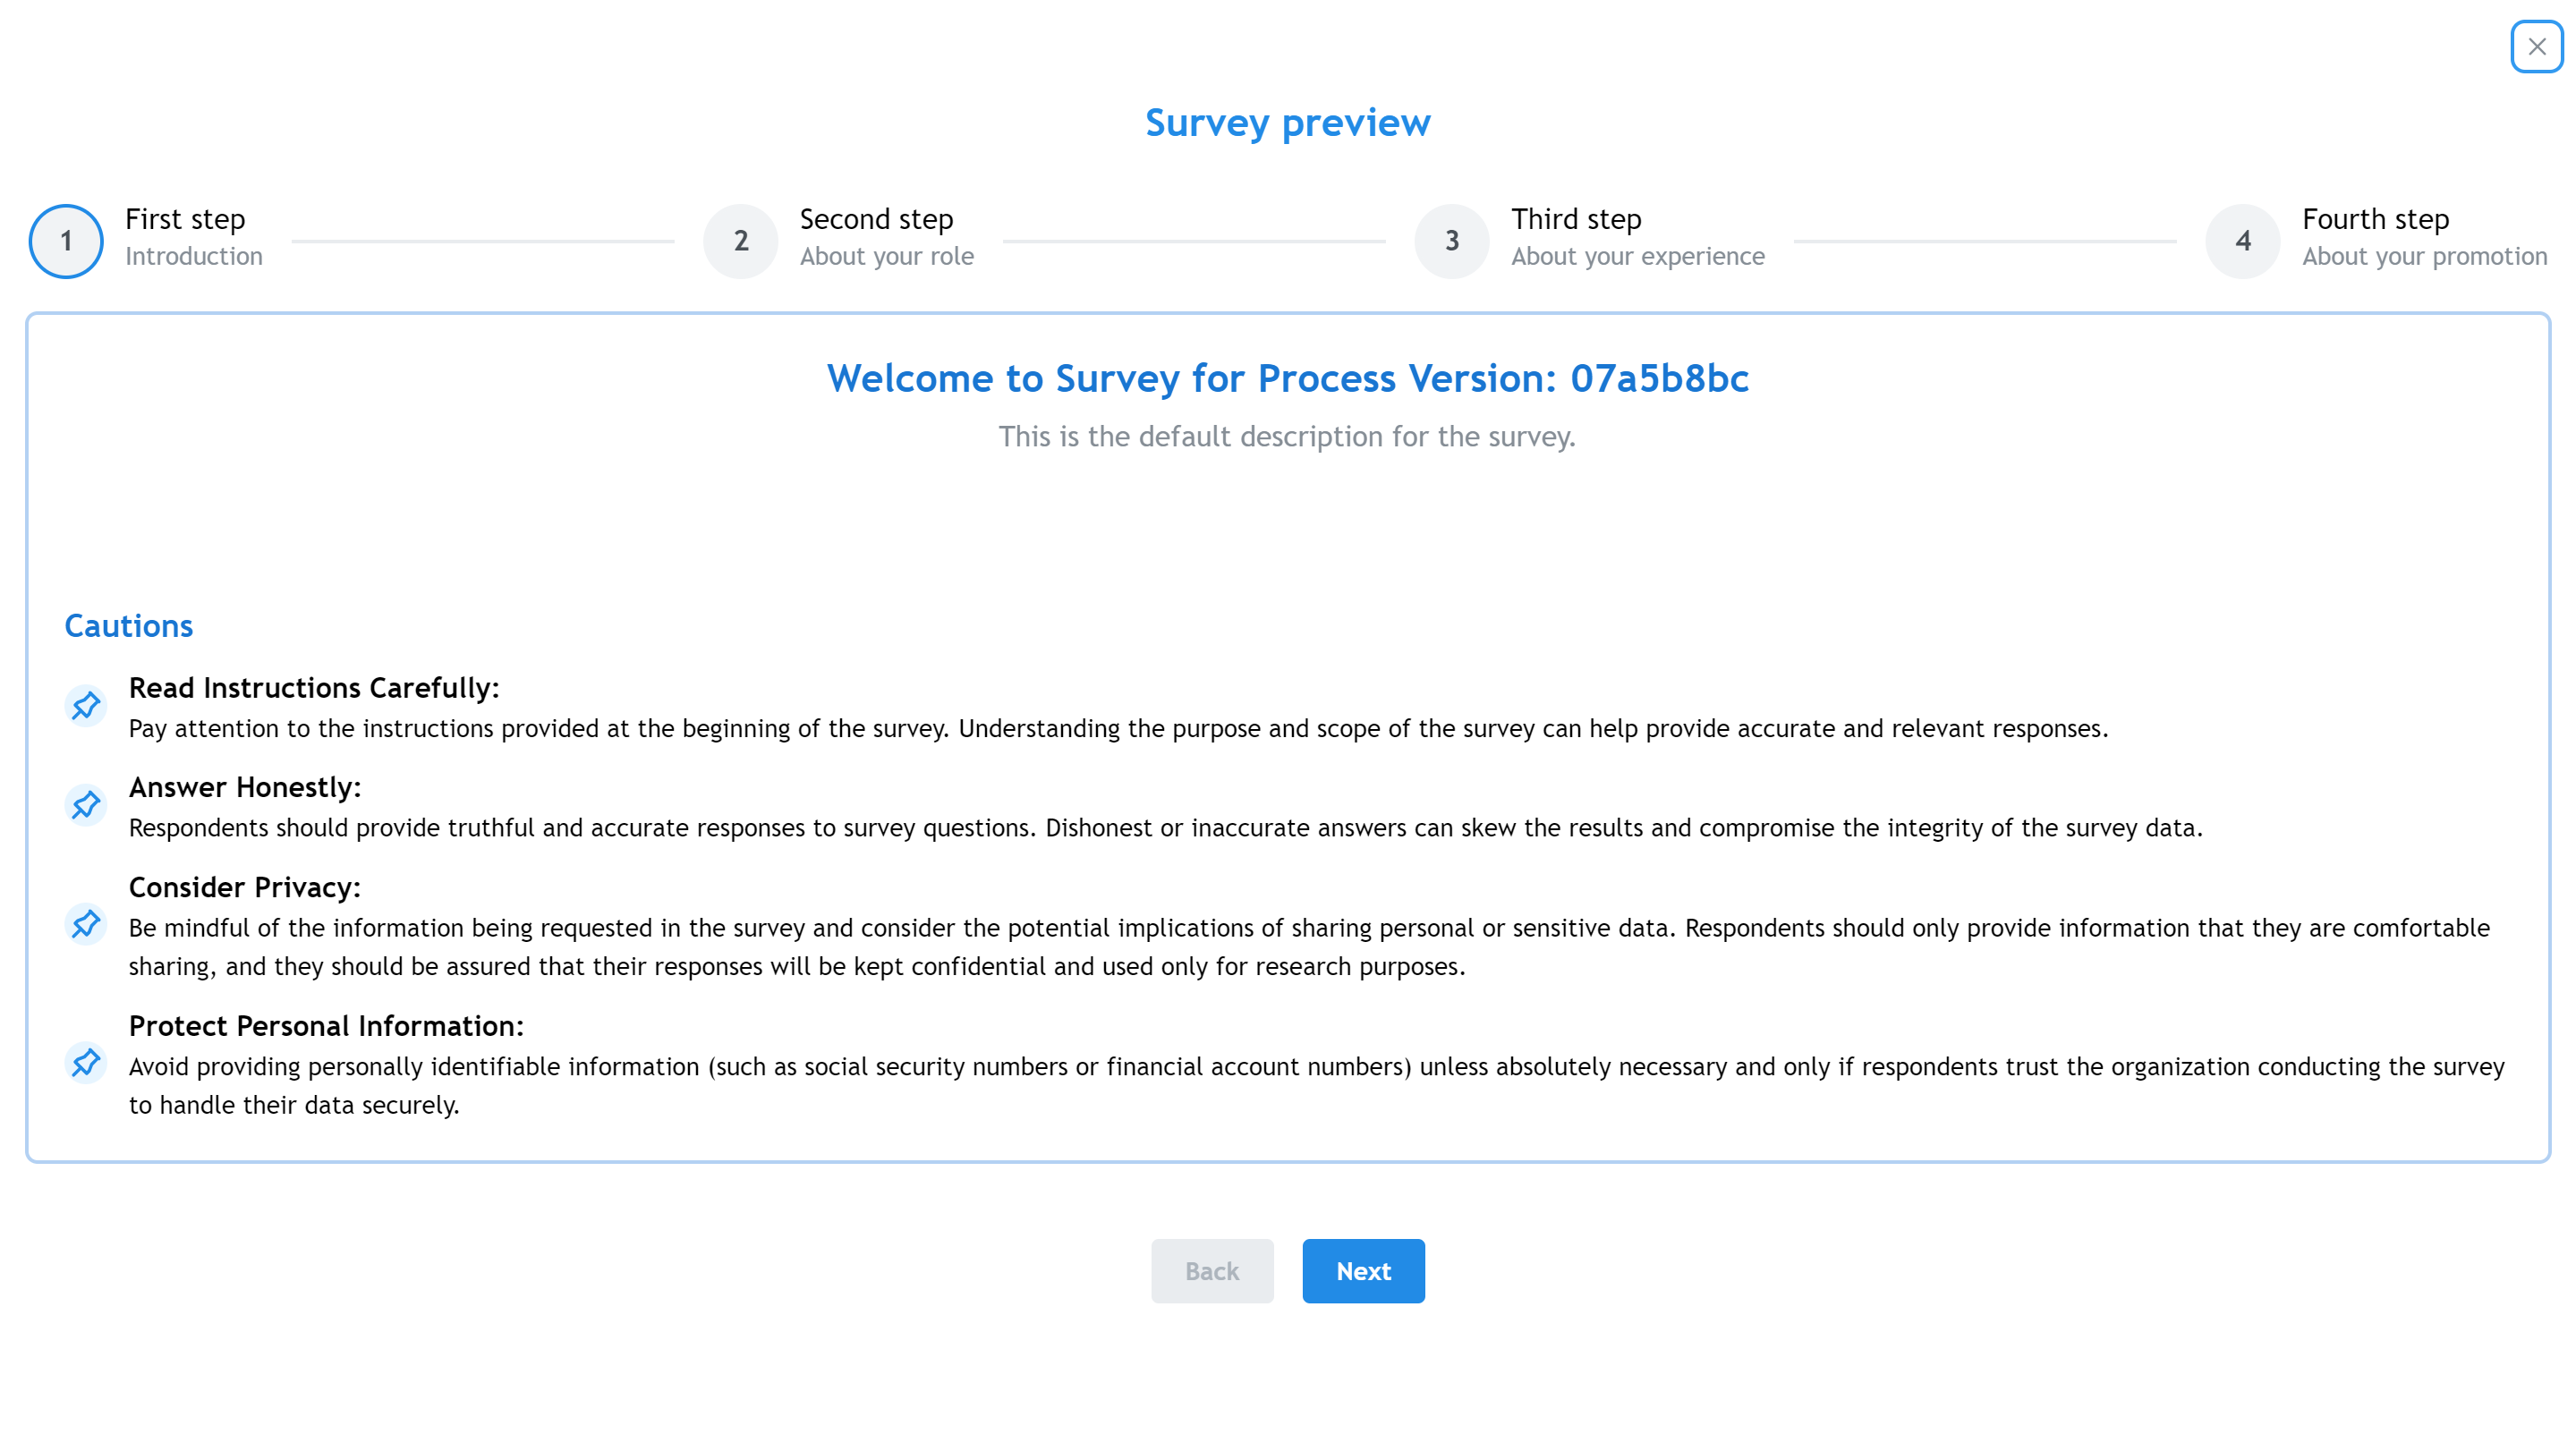
\includegraphics[ width = \linewidth]{Content/Hiện thực hệ thống/documents/Hiện thực giao diện người dùng/images/SurveyPreviewIntroduction.png}
    \vspace{0.5cm}
    \caption{Giao diện xem trước bảng khảo sát - trang mở đầu}
    \label{fig: Giao diện xem trước bảng khảo sát - trang mở đầu}
\end{figure}

Trang mở đầu của bảng khảo sát sẽ hiển thị thông tin chung của bảng khảo sát như tên, mô tả, những cảnh báo đối với người làm khảo sát. Để chuyển đến phần tiếp theo người dùng chọn nút Next, tương tự nếu muốn quay trở lại phần trước đó thì có thể chọn Back.

\begin{figure}[H]
    \centering
    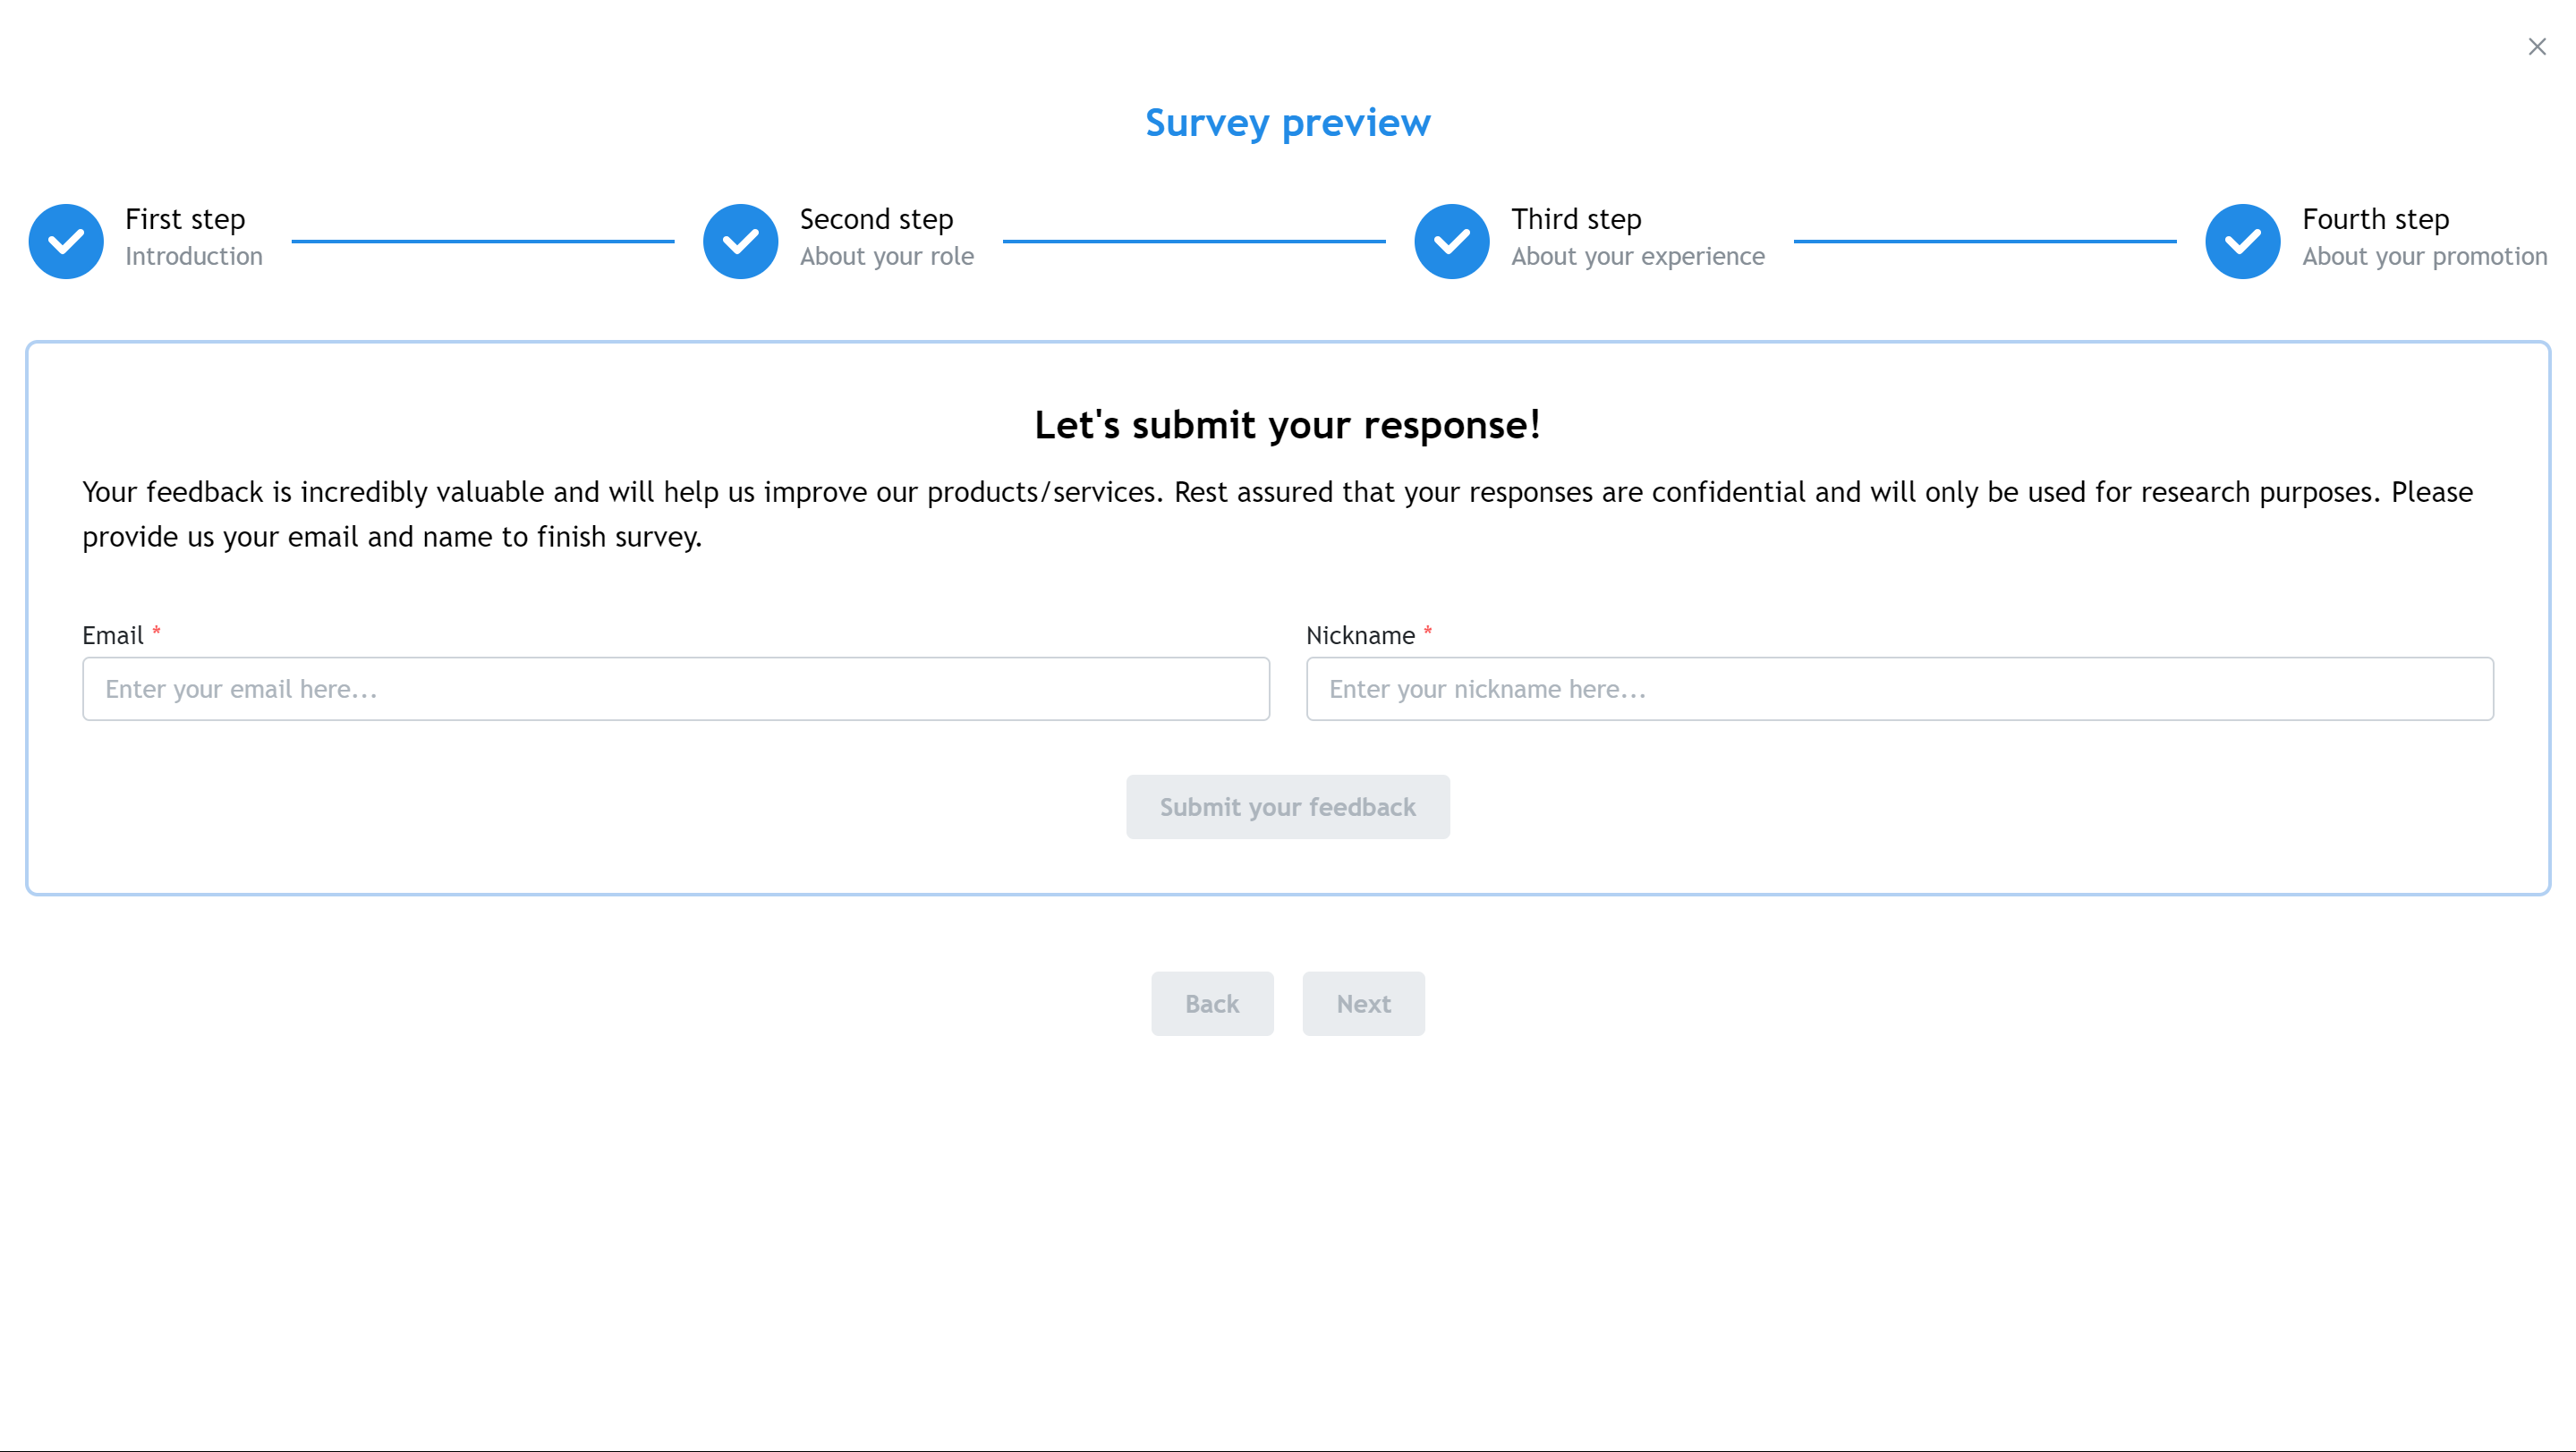
\includegraphics[ width = \linewidth]{Content/Hiện thực hệ thống/documents/Hiện thực giao diện người dùng/images/SurveyPreviewConclusion.png}
    \vspace{0.5cm}
    \caption{Giao diện xem trước bảng khảo sát - trang kết thúc}
    \label{fig: Giao diện xem trước bảng khảo sát - trang kết thúc}
\end{figure}

Trang kết thúc của bảng khảo sát sẽ hiển thị lời cảm ơn và yêu cầu người dùng nhập thông tin như tên và email để nhận được kết quả của bảng khảo sát sau khi khảo sát đóng. Sau khi nhập đầy đủ thông tin thì người dùng chọn nút Submit để gửi đi phản hồi bảng khảo sát.